\section{LwM2M - Lightweight M2M}
\subsection{Einführung}
LwM2M ist ein speziell für IoT entwickeltes Management- und Messaging-Protokoll. Wie es der Name schon verrät, handelt es sich um ein M2M - Machine-to-Machine Protokoll. Bei LwM2M wird ein Client-Server-Modell umgesetzt. Dabei werden alle Daten per Request angefragt und als Response beantwortet.

Entwickelt und standardisiert wurde dieses durch die Open Mobile Alliance, kurz OMA. Die Oma ist ein Verbund aus Firmen, welche in der Mobilfunksparte tätig sind, wie zum Beispiel Nokia, Motorola oder auch viele grosse Mobilfunkprovider. 

\subsection{Protocol Stack}

LwM2m ist ein Applikationslayer Protokoll und hat als Basis das CoAP Protokoll. Alle LwM2M Befehle werden umgewandelt, damit diese über CoAP zum Geräte gesendet werden. Dabei werden nicht alle Features von CoAP eingesetzt und unterstützt. CoAP ist wie auch LwM2M speziell für M2M (Maschine-to-Machine) Applikationen entwickelt worden.

Unterhalb von CoAP gibt es drei Varianten, die am gebräuchlichsten sind. UDP, UDP mit DTLS und SMS. Verwendet man nur UDP wird keine Verschlüsselung verwendet. Alle Daten werden in Klartext übertragen. Um eine sichere Verbindung herzustellen muss DTLS eingerichtet werden. Zusätzlich gibt es noch die Möglichkeit SMS. Diese ist speziell für Geräte ohne Internetanschluss gedacht. Alle Anfragen werden in ein SMS gepackt und so über das Telekommunikationsnetz übertragen.

Unterhalb der Verbindungsschicht können wieder viele verschiedene Technologien eingesetzt werden. Dies ist unter anderem IPv4, IPv6, 6LoWPAN oder auch ZigBee IP. 

Mit all diesen Möglichkeiten bietet LwM2M eine grosse Abdeckung an Technologien und kann vielseitig eingesetzt werden. 
\begin{figure}[H]
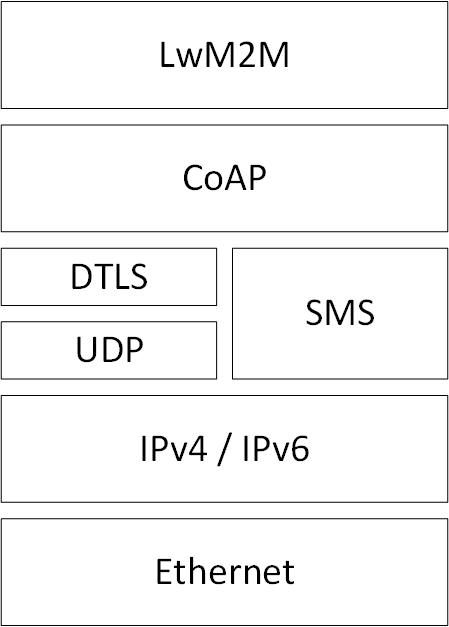
\includegraphics[scale=0.3]{images/lwm2m/stack.png}
\caption{LwM2M Stack}
\end{figure}

\subsection{Client-Server Model}
Die drei zentralen Bestandteil des Protokolls sind der Bootstrap-Server der LwM2M-Server und der LwM2M-Client. Der Bootstrap-Server ist für den Erstkontakt sowie die Erstkonfiguration zuständig. Die restliche Kommunikation läuft zwischen dem LwM2M-Server und dem LwM2M-Client. Ohne einen Bootstrap-Server kommunizieren die Geräte direkt mit dem LwM2M-Server.
\subsubsection{Client}
Der Client kann viele verschiedene Formen annehmen. Ein Beispiel wäre eine Linux Installation auf einem Raspberry Pi, welche einen Java LwM2M Client gestartet hat. An dem Raspberry Pi kann man nun mehrere Sensoren, wie Temperatur, Druck, etc. anschliessen und diese über den Client steuern. Es kann sich aber auch nur um einen kleinen Chip mit Sensor handeln, welcher ein C LwM2M Client beinhaltet. Client Umsetzungen gibt es dabei in den Programmiersprachen C und Java.
\subsubsection{Server}
Die Serverumsetzung ist sehr ähnlich wie die Clientumsetzung. Es wird auf einem Server eine Serverinstanz gestartet und diese wartet auf Clients, welche sich Registrieren möchten. Da die Serverimplementierung, wie auch der Client in C und Java verfügbar ist, gibt es viele Möglichkeiten den Server zu deployen. So kann er auf einer Windows- sowie auch unter Linux gestartet werden. Der Server hört dann auf dem CoAP Port auf die Anfragen.
\subsubsection{Management Server}
Der Management Server klinkt sich nun beim LwM2M Server ein. Dieser Server kann direkt oder über ein Web API angesprochen werden. Je nach Implementierung gibt es beide Varianten. So könnte man mehrere Serverinstanzen zu einem Management Server hinzufügen, um alles zentral Verwalten zu können. Möchte man nun ein Gerät managen, schickt man einen Befehl an den zuständigen LwM2M Server und dieser leitet den Befehl nun an das Device weiter. Die Antwort wird danach bis zum Management Server zurückgegeben und ausgewertet. 
\subsubsection{Bootstrap-Server}
Um ein ''factory bootstrap'' zu vermeiden, hat LwM2M einen Bootstrap-Server. Dieser ist für die Erstkonfiguration Zuständig und macht die Geräte variabler einsetzbar. Auf der Grafik ist dieser nicht erfasst worden. Wichtige Einstellungen die der Bootstrap-Server verteilen kann sind unter anderen\cite{BootstrapFeatures}:
\begin{itemize}
\item Keys  und Zertifikate für DTLS
\item Server URL
\item SMS Security Parameter
\item Kommunikationsparameter
\item Access Control Lists
\end{itemize}
Durch den Einsatz von Bootstraping nimmt man sich viel Managementarbeit ab und hat ein einheitlicheres und besser verwaltetes Netzwerk von LwM2M-Server und Client.
\begin{figure}[H]
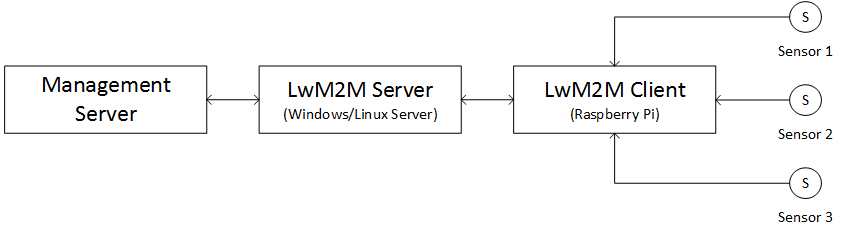
\includegraphics[scale=0.5]{images/lwm2m/server_client_model.png}
\caption{Client-Server-Model}
\end{figure}

\subsection{Object Model}
Eine klare Stärke des LwM2M-Protokolls sind die Object Models. Durch die Object Models werden alle Informationen eines Devices in einem strukturierten Model abgelegt, damit ein geregelter Zugriff auf alle Daten entsteht. Es wird zwischen Model und Ressource unterschieden. Eine Ressource ist zum Beispiel der Temperaturwert eines Temperatursensors. Eine zusätzliche Ressource könnte die dazugehörige Temperatureinheit sein. Mehrere solche Ressourcen werden zu einem Object Model zusammengefasst.

\subsection{Aufbau}
Jedes Object Model besitzt eine eindeutige Identifikationsnummer. Diese geht von 0-32768 und sind folgendermassen verteilt:
\begin{itemize}
\item 0-1023: OMA-Label
\item 1024-2047: Reserviert für zukünftige Benutzung
\item 2048-10240: Registrierungen der Partnerfirmen
\item 10241-32768: Individuelle Registrierungen durch Firmen oder Personen
\end{itemize}
Wenn man ein neues Model erstellen möchte, geht man auf die OMA-Seite und erfasst dieses im ''LWM2M Management Object Editor''. Pro neuem Modell muss man eine ID, Namen, ObjectVersion, LWM2MVersion, Object URN, Instances und Mandatory festlegen. Mit Instances gibt man an, ob ein Object pro Device mehrmals vorhanden sein darf.

Pro Object Model können nun die Ressourcen hinzugefügt werden. Diese besitzen auch eine eindeutige Identifikationsnummer von 0 bis 32768. Hier gibt es folgende Unterteilung:
\begin{itemize}
\item 0-2047: Common Ressources
\item 2048-26240: Reusable Ressources
\item 26241-32768: Private Ressources
\end{itemize}

Durch all diese Standardisierten Objekte und Ressourcen kann man jede Information eines Gerätes beschreiben und es entstehen keine Kompatibilitätsprobleme.

\subsubsection{Beispiel XML}
Hier sieht man ein Beispiel von dem Object Model ''Device'' mit der Ressource ''0 - Manufacturer''. Das Object Model besitzt aber noch weitere Ressourcen, die andere Informationen eines Devices definieren.
\begin{lstlisting}[%
language=xml]
<LWM2M>
	<Object">
		<Name>Device</Name>
		<Description1><![CDATA[ This LWM2M Object ... ]]></Description1>
		<ObjectID>3</ObjectID>
		<ObjectURN>TBD</ObjectURN>
		<MultipleInstances>Single</MultipleInstances>
		<Mandatory>Mandatory</Mandatory>
		<Resources>
			<Item ID="0">
				<Name>Manufacturer</Name>
				<Operations>R</Operations>
				<MultipleInstances>Single</MultipleInstances>
				<Mandatory>Optional</Mandatory>
				<Type>String</Type>
				<RangeEnumeration />
				<Units/>
				<Description><![CDATA[ Human rea... ]]</Description>
			</Item>
			<Item>...</Item>
		</Resources>
	</Object>
</LWM2M>
\end{lstlisting}

\begin{figure}[H]
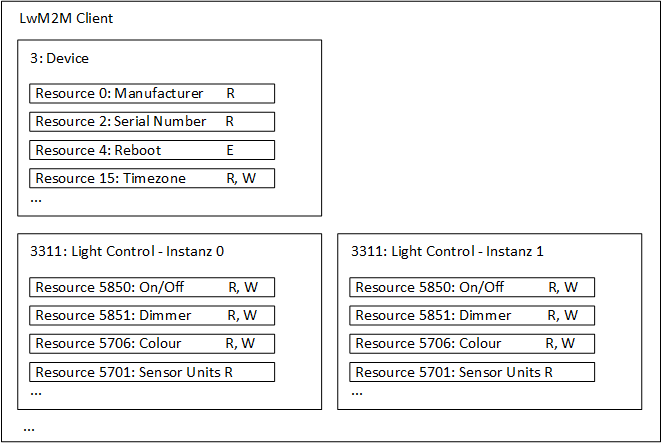
\includegraphics[scale=0.65]{images/lwm2m/lwm2m_client.png}
\caption{LwM2M Stack}
\end{figure}

xml

Standarts + eigene

\section{Features und Funktionen}

\subsection{Bootstrapping}
\begin{figure}[H]
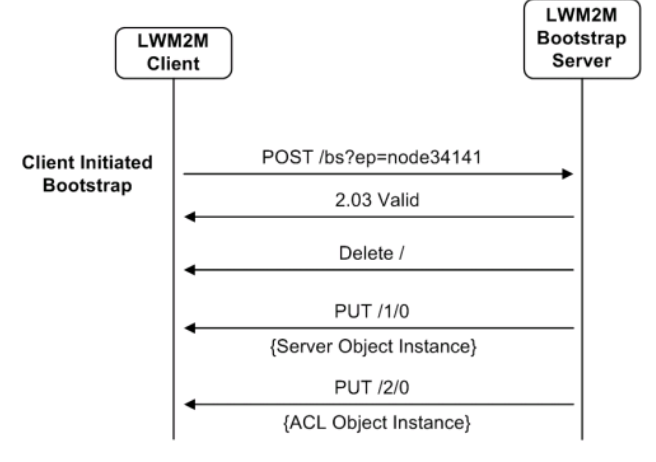
\includegraphics[scale=0.5]{images/lwm2m/bootstrap_diagram.png}
\caption{LwM2M Stack\cite{LwM2MInterfaces}}
\end{figure}
Pre-Configured, Server initial Bootstrap

\subsection{Registration}

\begin{figure}[H]
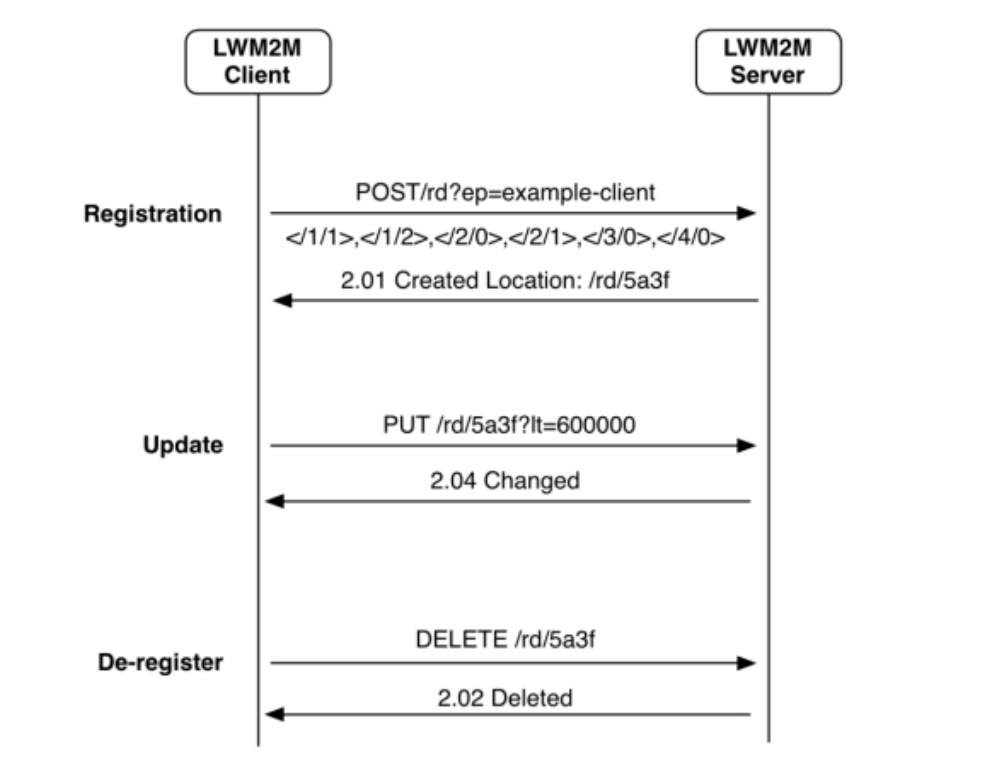
\includegraphics[scale=0.5]{images/lwm2m/registration_diagram.png}
\caption{LwM2M Stack\cite{LwM2MInterfaces}}
\end{figure}
Resource discovery
register, update, de-register


\subsection{Object / Resource Access}
\begin{figure}[H]
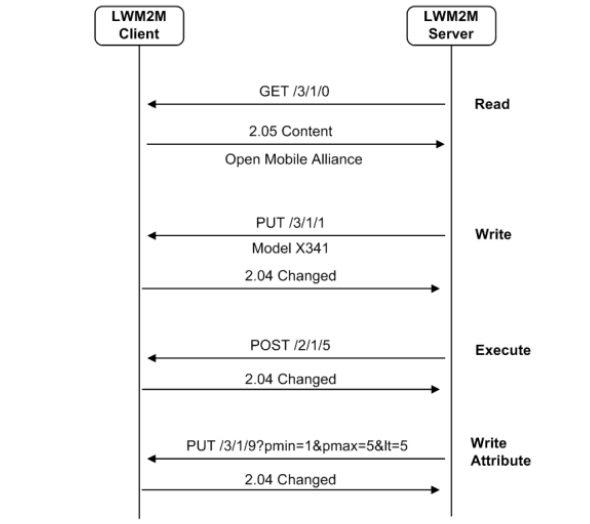
\includegraphics[scale=0.5]{images/lwm2m/command_diagram.png}
\caption{LwM2M Stack\cite{LwM2MInterfaces}}
\end{figure}

Management Objects and Resources
CoAP Rest api
read, write, execute, create, delete

\subsection{Reporting}

\begin{figure}[H]
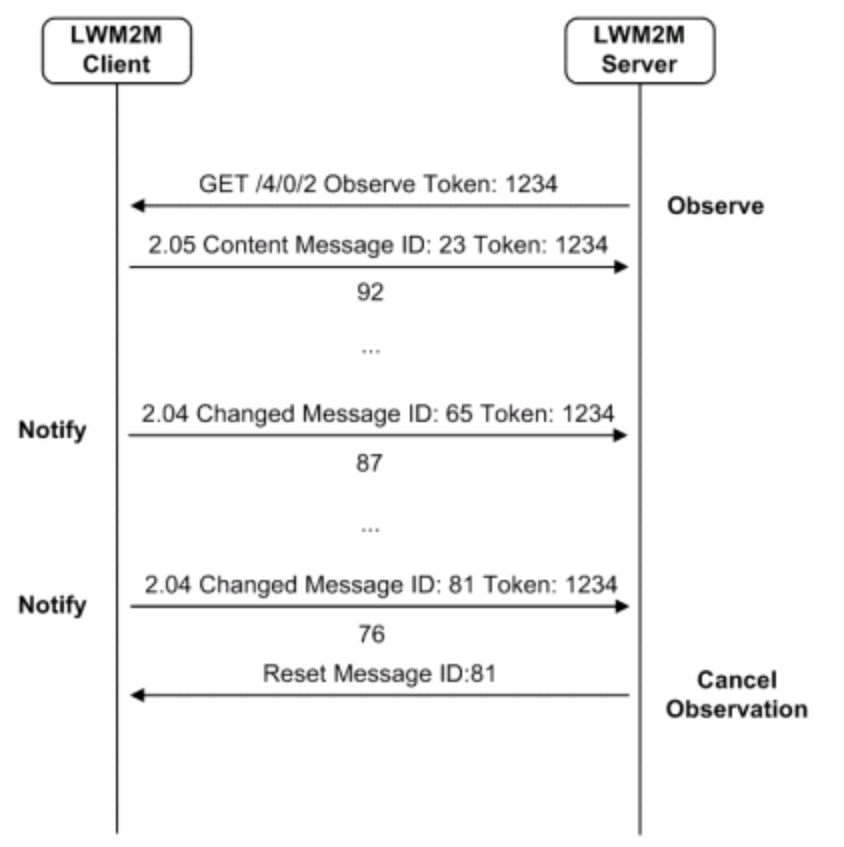
\includegraphics[scale=0.5]{images/lwm2m/report_diagram.png}
\caption{LwM2M Stack\cite{LwM2MInterfaces}}
\end{figure}
Observing
observe,cancal observe,  notify
